%%%%%%%%%%%%%%%%%%%%%%%%%%%%%%%%%%%%%%%%%
% Short Sectioned Assignment
% LaTeX Template
% Version 1.0 (5/5/12)
%
% This template has been downloaded from:
% http://www.LaTeXTemplates.com
%
% Original author:
% Frits Wenneker (http://www.howtotex.com)
%
% License:
% CC BY-NC-SA 3.0 (http://creativecommons.org/licenses/by-nc-sa/3.0/)
%
%%%%%%%%%%%%%%%%%%%%%%%%%%%%%%%%%%%%%%%%%

%----------------------------------------------------------------------------------------
%	PACKAGES AND OTHER DOCUMENT CONFIGURATIONS
%----------------------------------------------------------------------------------------

\documentclass[paper=a4, fontsize=11pt]{scrartcl} % A4 paper and 11pt font size

\usepackage[T1]{fontenc} % Use 8-bit encoding that has 256 glyphs
\usepackage{fourier} % Use the Adobe Utopia font for the document - comment this line to return to the LaTeX default
\usepackage[english]{babel} % English language/hyphenation
\usepackage{amsmath,amsfonts,amsthm} % Math packages

\usepackage{sectsty} % Allows customizing section commands
\usepackage[top=5em]{geometry}
\allsectionsfont{\centering \normalfont\scshape} % Make all sections centered, the default font and small caps

\usepackage{fancyhdr} % Custom headers and footers
\pagestyle{fancyplain} % Makes all pages in the document conform to the custom headers and footers
\fancyhead{} % No page header - if you want one, create it in the same way as the footers below
\fancyfoot[L]{} % Empty left footer
\fancyfoot[C]{} % Empty center footer
\fancyfoot[R]{\thepage} % Page numbering for right footer
\renewcommand{\headrulewidth}{0pt} % Remove header underlines
\renewcommand{\footrulewidth}{0pt} % Remove footer underlines
\setlength{\headheight}{5pt} % Customize the height of the header

\numberwithin{equation}{section} % Number equations within sections (i.e. 1.1, 1.2, 2.1, 2.2 instead of 1, 2, 3, 4)
\numberwithin{figure}{section} % Number figures within sections (i.e. 1.1, 1.2, 2.1, 2.2 instead of 1, 2, 3, 4)
\numberwithin{table}{section} % Number tables within sections (i.e. 1.1, 1.2, 2.1, 2.2 instead of 1, 2, 3, 4)

\setlength\parindent{0pt} % Removes all indentation from paragraphs - comment this line for an assignment with lots of text

\usepackage{mathtools}
\usepackage{amssymb}
\usepackage{gensymb}
\usepackage{chngcntr}
\counterwithout{figure}{section}
%----------------------------------------------------------------------------------------
%	TITLE SECTION
%----------------------------------------------------------------------------------------

\newcommand{\horrule}[1]{\rule{\linewidth}{#1}} % Create horizontal rule command with 1 argument of height

\title{	
\normalfont \normalsize 
\textsc{Utah State University, Computer Science Department} \\ [25pt] % Your university, school and/or department name(s)
\horrule{0.5pt} \\[0.4cm] % Thin top horizontal rule
\huge CS 7910 Computational Complexity\\Homework 1 \\ % The assignment title
\horrule{2pt} \\[0.5cm] % Thick bottom horizontal rule
}

\author{Gopal Menon} % Your name

\date{\normalsize\today} % Today's date or a custom date

\begin{document}

\maketitle % Print the title

\begin{figure}[!h]
\centering
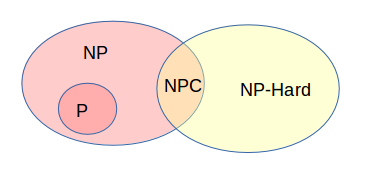
\includegraphics[width=3.5in]{P-NP.png}
\caption{P, NP, NP-Complete (NPC) and NP-Hard problems}
\label{P-NP}
\end{figure}

\begin{enumerate}
  \item \textit{For each of the following statements, please tell whether it is true and briefly explain your answer.}
  \begin{enumerate}
    \item \textit{If there exists a polynomial time algorithm that can solve the circuit satisfiability problem, then every problem in $NPC$ can be solved in polynomial time.}
    
The circuit satisfiability ($CSAT$) problem is NP-Complete. This means that
\begin{enumerate}
\item $CSAT \in NP$ and
\item for all problems $Y \in NP$, $Y \leq_P CSAT$ 
\end{enumerate}
This means that every problem $Y$ in $NP$ can be reduced to $CSAT$. Or in other words, $CSAT$ is at least as hard as the hardest problem in $NP$. The set $NP-Complete$ is a subset of $NP$ as shown in figure \ref{P-NP}. So $CSAT$ is at least as hard as any $NP-Complete$ problem. This means that if if a polynomial time algorithm can be used to solve $CSAT$, then every other $NP-Complete$ problem can be solved in polynomial time since it would be easier or at most as difficult as $CSAT$.

    \item \textit{If no polynomial time algorithm can solve the SAT problem, then no polynomial time algorithm can solve the circuit satisfiability problem.}
    
    The $CSAT$ problem can be reduced to the $SAT$ problem as we saw in class. This means that $CSAT \leq_P SAT$. i.e. the $SAT$ problem is at least as hard if not harder than $CSAT$. If no polynomial time algorithm can be used to solve the $SAT$ problem, it does not follow from this that no polynomial time algorithm can be used to solve the $CSAT$ problem. However since all $NP$ problems can be reduced to an $NP-Complete$ problem, and since we know that $CSAT$ is an $NP-Complete$ problem, it follows that $SAT \leq_P CSAT$. Since no polynomial time algorithm can be used to solve the $SAT$ problem, it follows that no polynomial time algorithm can be used to solve the $CSAT$ problem which is at least as hard as the $SAT$ problem.
    
    \item \textit{$NP$ is the union of $P$ and $NPC$.}
    
    If $P=NP$ and since $NPC \subseteq NP$, in this case $NP = P \cup NPC$. But it is unlikely that $P=NP$. Since $NPC$ problems are the hardest $NP$ problems, the relation $NP = P \cup NPC$ can only be satisfied if $NP - P = NPC$. i.e. if each $NP$ problem that cannot be solved in polynomial time can be reduced to any other $NP$ problem in polynomial time.
    
    \item \textit{If there is an $NPC$ problem $A$ that is also in $P$, then $NP$ is the union of $P$ and $NPC$.}
    \item \textit{If no problem of $NPC$ is in $P$, then $NP$ is the union of $P$ and $NPC$.}
    \item \textit{If $NP$ is the union of $P$ and $NPC$, then $P=NP$.}
  \end{enumerate}
  
	\begin{figure}[!h]
		\centering
		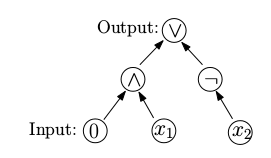
\includegraphics[width=2.5in]{CSAT.png}
		\caption{An instance of the circuit satisfiability problem}
		\label{CSAT}
	\end{figure}  
  
  \item \textit{In class we studied a polynomial time problem reduction from the circuit satisfiability problem to the SAT problem. The following figure shows an instance of the circuit satisfiability problem. Give the SAT problem instance constructed from it based on the problem reduction we studied in class, i.e., give the Boolean variables and the clauses for the SAT problem instance.}
\end{enumerate}


%----------------------------------------------------------------------------------------

\end{document}